\section{Capacity expansion strategies comparison}
%\subsection*{Capacity expansion strategies comparison}
%\addcontentsline{toc}{section}{Capacity expansion strategies comparison}
The previous section was related to the analysis of just the capacity expansion strategy created in this work. Now I am going to compare it to the rest of them and to test the impact that different capacity expansion strategies have on the development of the telecommunication infrastructure. The capacity expansion strategies are: \textit{\guillemotleft Minimum intervention\guillemotright , \guillemotleft Spectrum integration\guillemotright, \guillemotleft 700 MHz spectrum integration\guillemotright , \guillemotleft Small cells strategy\guillemotright, \guillemotleft Hybrid strategy\guillemotright }and\textit{ \guillemotleft 700 MHz densification\guillemotright }. These tests will use the baseline population growth scenario, the baseline user-speed growth scenario, and the \textit{\guillemotleft More profitable first\guillemotright} coverage obligation with a speed of 2 Mbps.\par

\subsection*{Population covered}
%\addcontentsline{toc}{subsection}{Population covered}
The population covered is the first output that we analyse. The following graph represents the evolution of the percentage covered per year and gives us an idea of the maximum percentage that the capacity expansion strategy is capable of providing in the given scenario. \par

%%%%%%%%%%%%%%%%%%%% Figure/Image No: 11 starts here %%%%%%%%%%%%%%%%%%%%

\begin{figure}[H]
	\begin{Center}
		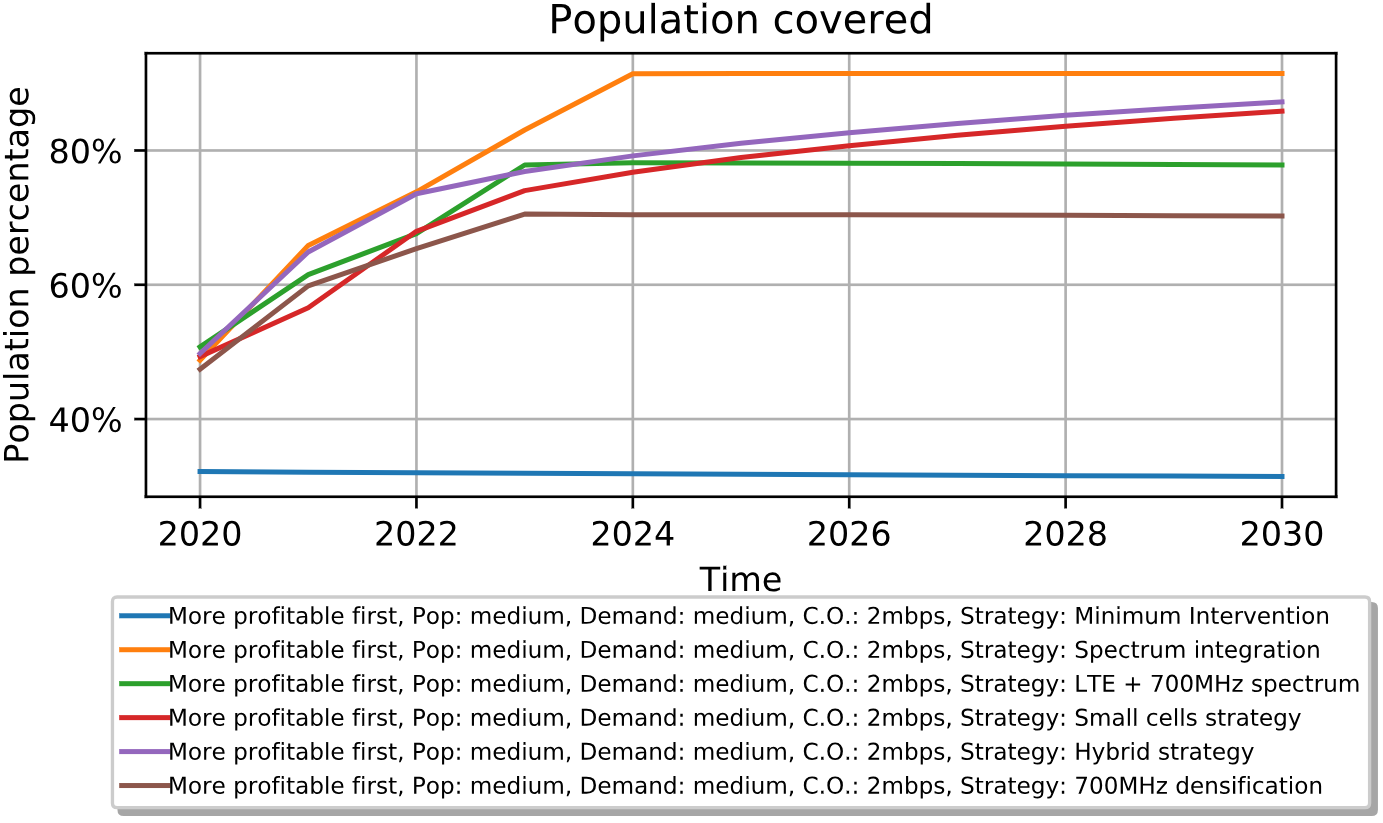
\includegraphics[width=0.95\textwidth]{./media/image50.png}
		\caption{Capacity strategies comparison. Graph: Population covered. Source: Author}
	\end{Center}
\end{figure}


%%%%%%%%%%%%%%%%%%%% Figure/Image No: 11 Ends here %%%%%%%%%%%%%%%%%%%%

This graph represents the population covered after the interventions of any one year. This way, the starting percentage is 32$\%$  and is the same for all the interventions. As can be seen in the plot, not all the lines reach 100$\%$  of the population covered by 2030. Apart from \textit{ \guillemotleft Minimum intervention\guillemotright}, that cannot build new assets and, therefore, does not increase the population covered, there are two main groups of strategies: those that can build new assets (\textit{\guillemotleft 700 MHz densification\guillemotright}, \textit{\guillemotleft Small cells strategy\guillemotright} and \textit{\guillemotleft Hybrid strategy\guillemotright}) and those that cannot (\textit{\guillemotleft Spectrum integration\guillemotright }and \textit{\guillemotleft 700 MHz spectrum integration\guillemotright}).\par

In the graph, only \textit{\guillemotleft Small cells strategy\guillemotright }and \textit{\guillemotleft Hybrid strategy\guillemotright} could potentially reach the 100$\%$  population covered while the rest only raise the percentage from 32$\%$  to 70-90$\%$ . This is because, while the small cells related strategies increase the percentage of population covered during the whole simulation, the rest stop growing around 2023-24. This is because of two factors: (I) the extremely good capacity of the small cells in the model and (II) that MINERVA allows densification strategies, which means creating more sites for small cells until all the demand is satisfied. If these strategies really achieve the 100$\%$  population covered will be studied later.\par

\textit{\guillemotleft 700 MHz densification\guillemotright} is also allowed to create new sites, but the 700 MHz band has less bandwidth than 3.7 GHz and, therefore, using only this band is not enough to meet the demand in some regions. Finally, the rest of the strategies are not allowed to create new sites, just to upgrade those sites that already have legacy technologies (Such as 2G and 3G). These strategies cannot satisfy the demand either but due to two different factors:\par

\begin{itemize}
	\item Checking the list of assets provided in the original model, there is a part of the PCDs that have no assets at the beginning of the execution in the whole PCD. This is not an issue of the behaviour of the code, but of the database from which this information was obtained for the NISMOD project. Half of the interventions (Except \textit{\guillemotleft Small cells strategy\guillemotright, \guillemotleft Hybrid strategy\guillemotright and \guillemotleft 700 MHz densification\guillemotright}) cannot build new assets, and, therefore, strategies that only use this type of interventions are affected by this limitation.\par

	\item The other factor is that there is a limit to the capacity that one band can provide. Strategies that only use one or two bands, such as \textit{\guillemotleft 700 MHz spectrum integration \guillemotright} and \textit{\guillemotleft 700 MHz densification\guillemotright} are mainly affected by this limitation in the most densely populated regions.
\end{itemize}\par

\textit{\guillemotleft Spectrum integration\guillemotright} strategy grows with the similar rate than the other macrocell related strategies, but when they stop growing, the \textit{\guillemotleft Spectrum integration\guillemotright }strategy continues the rise a little bit more and manages to reach around the 90$\%$  of the population. This is because it is the only strategy allowed to build assets with the 3,500 MHz band which has the bigger bandwidth and hence provides more capacity.\par

\subsection*{Investment}
%\addcontentsline{toc}{subsection}{Investment}
The second output that we will review is the comparison of costs. The following graph compares the investment effort that the telecom operator would make depending on the capacity expansion strategy. This graph also uses the baseline population growth scenario, the baseline user-speed growth scenario, and the \textit{\guillemotleft More profitable first\guillemotright} coverage obligation option with a speed of 2 Mbps.\par


%%%%%%%%%%%%%%%%%%%% Figure/Image No: 12 starts here %%%%%%%%%%%%%%%%%%%%

\begin{figure}[H]
	\begin{Center}
		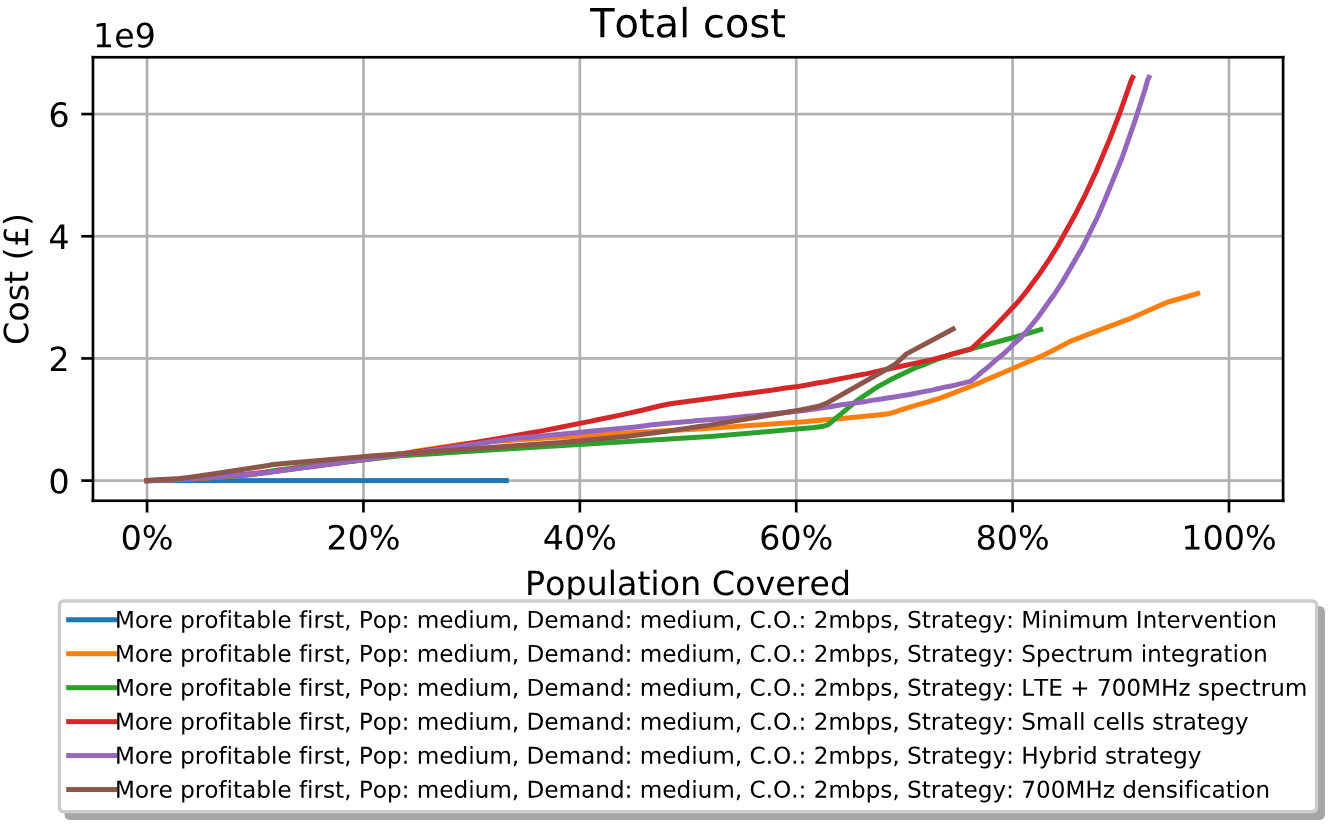
\includegraphics[width=0.95\textwidth]{./media/image51.png}
		\caption{Capacity strategies comparison. Graph: Total cost. Source: Author}
	\end{Center}
\end{figure}


%%%%%%%%%%%%%%%%%%%% Figure/Image No: 12 Ends here %%%%%%%%%%%%%%%%%%%%

The given graph represents the cost that takes to reach a specific population covered percentage for each capacity strategy. As can be seen in the plot, none of the lines reaches 100$\%$  since they cannot cover the whole population by 2030.\par

From the beginning to 75$\%$  covered, which are the urban and suburban areas, the marginal cost to increase by 1$\%$  is similar for most of the strategies. The $``$Small cells$"$  strategy is a little bit more expensive since it starts building small cells directly, while the rest of strategies use LTE or 700 MHz bands before. After 75$\%$  of the population, the cost of both small cells strategies grows drastically and makes it not affordable.\par

The graph also reflects the differences between all the strategies that only use macrocell bands (700, 800, 2,600, 3,500 MHz). \textit{\guillemotleft Spectrum integration\guillemotright} is the best strategy since can use all the bands and the only one that can use the 3,500 MHz band. Hence, the gap from 85$\%$  of the population covered to 95$\%$  is just thanks to adding this band, which helps in those regions where the rest of the bands combined were not enough. \textit{\guillemotleft 700 MHz spectrum integration\guillemotright }has LTE and 700 MHz, while \textit{\guillemotleft 700 MHz densification\guillemotright} only uses the 700 MHz. For this reason, despite \textit{\guillemotleft 700 MHz densification\guillemotright} can create new sites and can provide connectivity in places where it is not possible with the other strategies, \textit{\guillemotleft 700 MHz spectrum integration\guillemotright }is capable of covering much more population at the end of the execution. It is important to remember that these strategies are not limited by the budget of the operator, but by the technical issues explained above.\par


\subsection*{Capacity margin}
%\addcontentsline{toc}{subsubsection}{Capacity margin}
The capacity margin is the third and last output that we are going to evaluate, and it is related to the difference between the absolute value of the capacity of the network and the absolute value of the demand of the network in Mbps/km\textsuperscript{2}. This is not related to the coverage obligations, but to the estimated demand of the population. The following graph uses the baseline population growth scenario, the baseline user-speed growth scenario, and the \textit{\guillemotleft More profitable first\guillemotright} coverage obligation option with a speed of 2 Mbps.\par



%%%%%%%%%%%%%%%%%%%% Figure/Image No: 13 starts here %%%%%%%%%%%%%%%%%%%%

\begin{figure}[H]
	\begin{Center}
		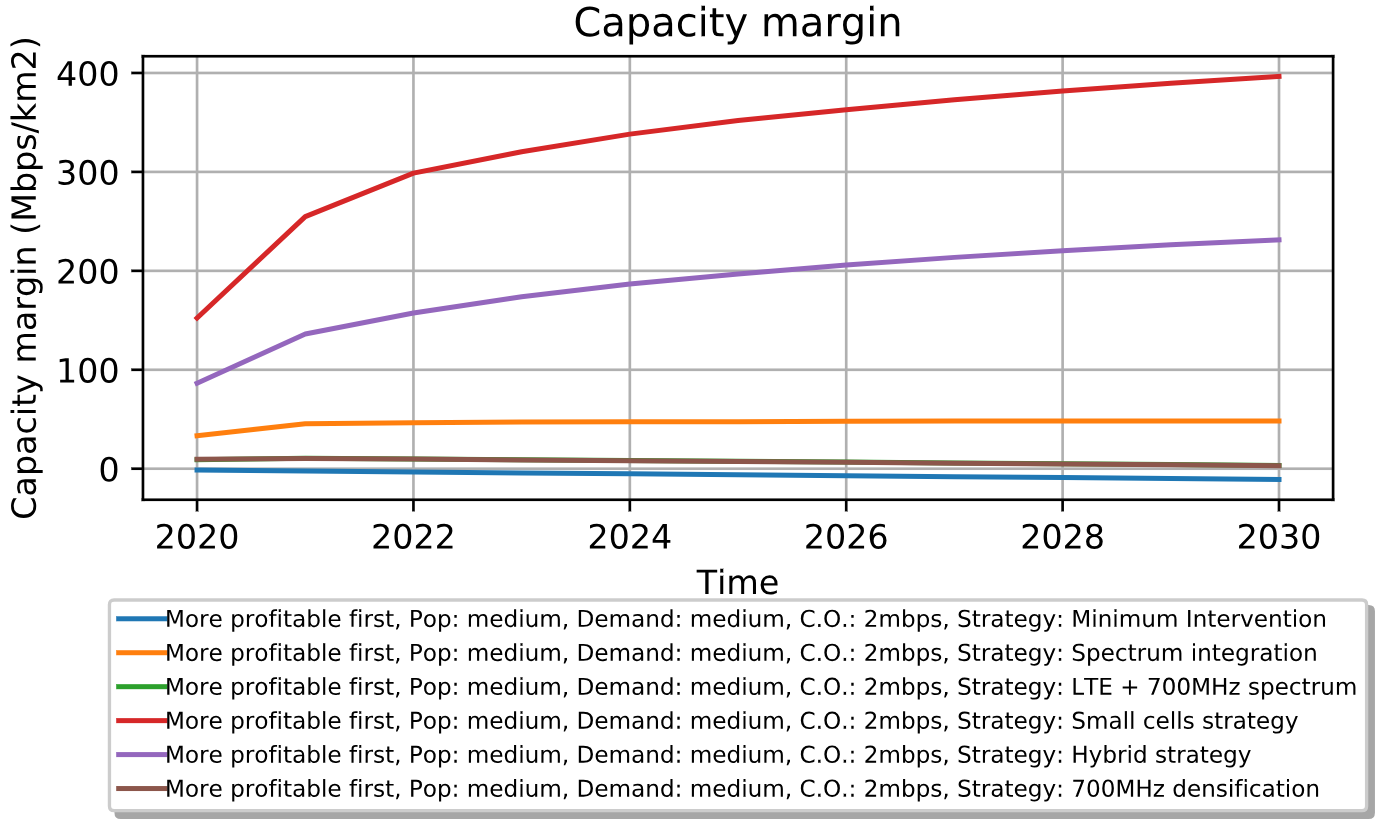
\includegraphics[width=0.95\textwidth]{./media/image52.png}
		\caption{Capacity strategies comparison. Graph: Capacity margin. Source: Author}
	\end{Center}
\end{figure}


%%%%%%%%%%%%%%%%%%%% Figure/Image No: 13 Ends here %%%%%%%%%%%%%%%%%%%%

The most interesting strategy for a telecom operator is to have high population covered, with the minimum cost possible and with a positive capacity margin but as small as possible. Otherwise, it would mean that the operator made a big investment that is not been harnessed. \par

This graph shows the same differences that we could see before. There is a strong difference between strategies that use the small cells intervention and those that do not. Small cells are good but expensive and using just small cells comprise a huge waste of budget in the less populated areas.\par

\subsection*{Total costs }
%\addcontentsline{toc}{subsection}{Total costs }
The model calculates that a telecom operator with a market share of 30$\%$  of the population that use mobile broadband services have approximately �600,000,000 per year to invest in new assets and operate them. The purpose of this section is to verify which of the limitations that we found in the previous charts are due to technical or monetary restrictions. In the case of the limitations that were because of the budget, this model also shows the total amount of money that would be needed.\par

The following chart represents the same information as the cost section, which is the cost that takes to achieve certain population covered, but removing the budget limitations:\par



%%%%%%%%%%%%%%%%%%%% Figure/Image No: 14 starts here %%%%%%%%%%%%%%%%%%%%

\begin{figure}[H]
	\begin{Center}
		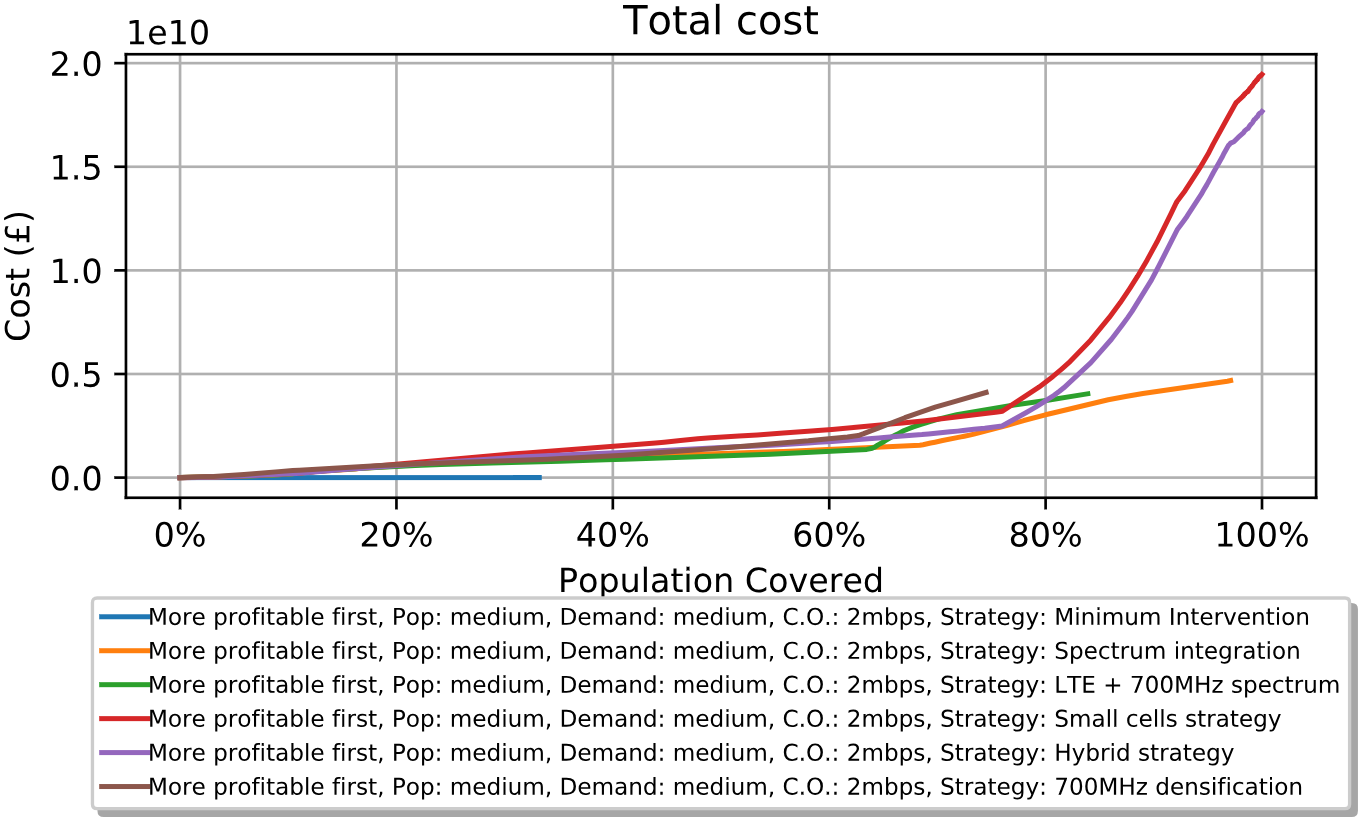
\includegraphics[width=0.95\textwidth]{./media/image53.png}
		\caption{Capacity strategies comparison. Graph: Total cost without budget limitation. Source: Author}
	\end{Center}
\end{figure}


%%%%%%%%%%%%%%%%%%%% Figure/Image No: 14 Ends here %%%%%%%%%%%%%%%%%%%%

As can be seen, the graph is similar to the previous one, but now the \textit{\guillemotleft Small cells strategy\guillemotright} and the \textit{\guillemotleft Hybrid strategy\guillemotright} strategies reach the 100$\%$  population covered, which confirms the previous analysis. \par

The maximum budget that the operator can spend in 11 years (From 2020 to 2030) is �6,600,000,000 which was the maximum value of the Y-axis in the budget limited cost chart. Now, the total cost is �20,600,000,000 which is three times the budget that the operator has. In fact, it is also important to remark that rising the population covered from 90$\%$  to 100$\%$  implies spending more than two times of what it took to rise from the original coverage to 90$\%$ .\par

The rest of strategies are not modified since they were not limited by budget but by technical constraints.\par

The capacity margin is also affected in this case and the results are not good for the small cells since the final capacity margin is too big. The following graph represents the capacity margin per year. As the budget is not limited, the operator builds all the assets in 2020, but it shows the differences between strategies clearly. \par



%%%%%%%%%%%%%%%%%%%% Figure/Image No: 15 starts here %%%%%%%%%%%%%%%%%%%%

\begin{figure}[H]
	\begin{Center}
		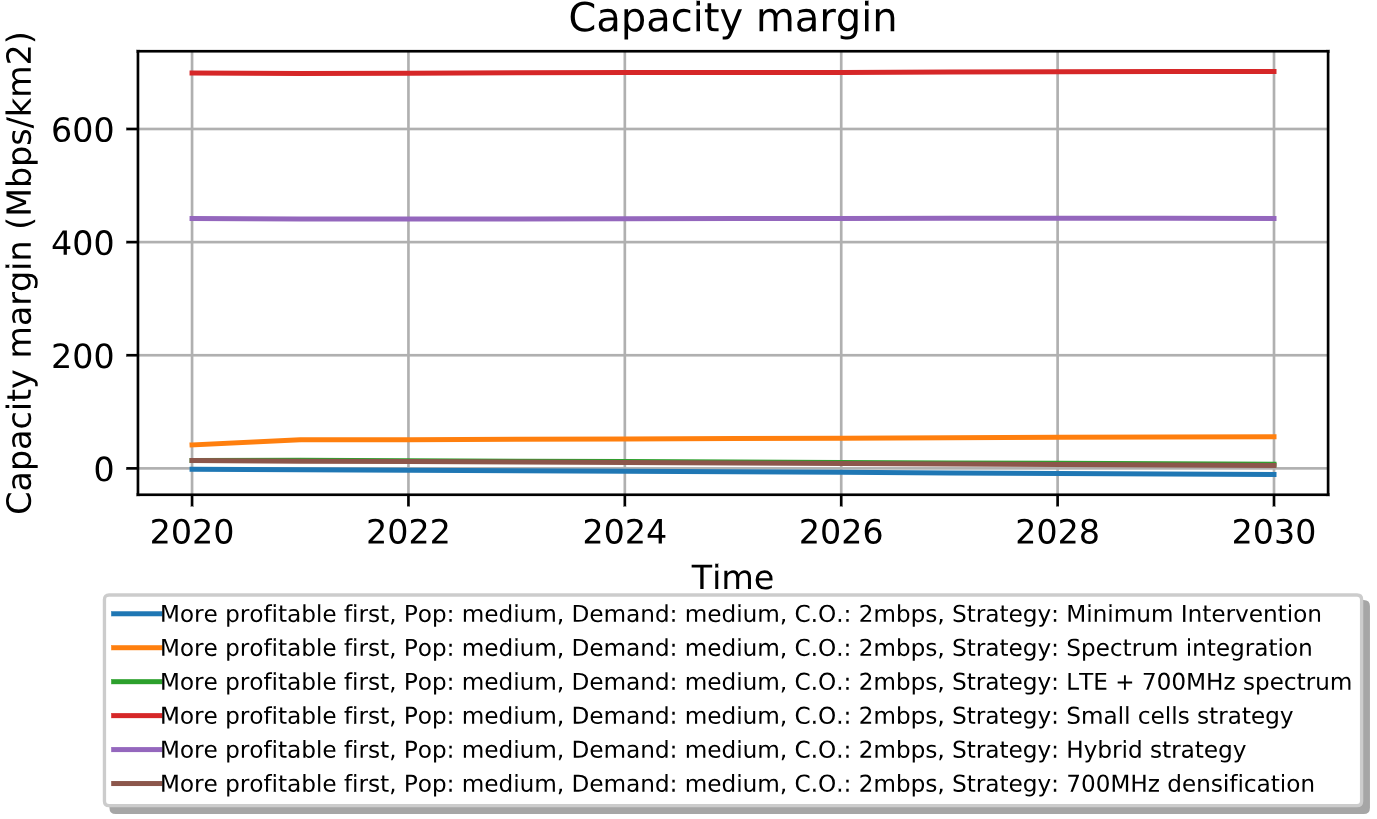
\includegraphics[width=0.95\textwidth]{./media/image54.png}
		\caption{Capacity strategies comparison. Graph: Capacity margin without budget limitation. Source: Author}
	\end{Center}
\end{figure}


%%%%%%%%%%%%%%%%%%%% Figure/Image No: 15 Ends here %%%%%%%%%%%%%%%%%%%%

The important point of this graph is that it allows us to see which is the maximum capacity margin for each capacity expansion strategy. In the previous capacity margin graph, the small cells related strategies did not stop growing their margin. In this graph, we can see the real final value of the strategies. However, the rest of the strategies do not increase their margin in spite of having an unlimited budget. This is mainly because these strategies have a technical limitation, not a budget limitation. \par

